%%%%%%%%%%%%%%%%%%%%%%%%%%%%%%%%%%%%%%%%%%%%%%%%%%%%%%%%%%%%%%%%%%%%%%%%%%%%%%%%%%%%%%%%%%
% Ceci est le fichier principal du template template à utiliser pour les rapports du     %
% projet 1 (Construction de Programme) d'INFO0947.                                       %
%                                                                                        %
% Vous devez décommenter et compléter les commandes introduites plus bas (intitule, ...) %
% avant de pouvoir compiler le fichier LaTeX.  Pensez à configurer votre Makefile en     %
% conséquence.                                                                           %
%                                                                                        %
% Le contenu et la structure du rapport sont imposés.  Vous devez compléter les          %
% différents fichiers .tex inclus dans ce fichier avec votre production.                 %
%%%%%%%%%%%%%%%%%%%%%%%%%%%%%%%%%%%%%%%%%%%%%%%%%%%%%%%%%%%%%%%%%%%%%%%%%%%%%%%%%%%%%%%%%%

% !TEX root = ./main.tex
% !TEX engine = latexmk -pdf
% !TEX buildOnSave = true
\documentclass[a4paper, 11pt, oneside]{article}

\usepackage[utf8]{inputenc}
\usepackage[T1]{fontenc}
\usepackage[french]{babel}
\usepackage{array}
\usepackage{shortvrb}
\usepackage{listings}
\usepackage[fleqn]{amsmath}
\usepackage{amsfonts}
\usepackage{fullpage}
\usepackage{enumerate}
\usepackage{graphicx}             % import, scale, and rotate graphics
\usepackage{subfigure}            % group figures
\usepackage{alltt}
\usepackage{url}
\usepackage{indentfirst}
\usepackage{eurosym}
\usepackage{listings}
\usepackage{color}
\usepackage[table,xcdraw,dvipsnames]{xcolor}

% Change le nom par défaut des listing
\renewcommand{\lstlistingname}{Extrait de Code}


\definecolor{mygray}{rgb}{0.5,0.5,0.5}
\newcommand{\coms}[1]{\textcolor{MidnightBlue}{#1}}

\lstset{
    language=C, % Utilisation du langage C
    commentstyle={\color{MidnightBlue}}, % Couleur des commentaires
    frame=single, % Entoure le code d'un joli cadre
    rulecolor=\color{black}, % Couleur de la ligne qui forme le cadre
    stringstyle=\color{RawSienna}, % Couleur des chaines de caractères
    numbers=left, % Ajoute une numérotation des lignes à gauche
    numbersep=5pt, % Distance entre les numérots de lignes et le code
    numberstyle=\tiny\color{mygray}, % Couleur des numéros de lignes
    basicstyle=\tt\footnotesize,
    tabsize=3, % Largeur des tabulations par défaut
    keywordstyle=\tt\bf\footnotesize\color{Sepia}, % Style des mots-clés
    extendedchars=true,
    captionpos=b, % sets the caption-position to bottom
    texcl=true, % Commentaires sur une ligne interprétés en Latex
    showstringspaces=false, % Ne montre pas les espace dans les chaines de caractères
    escapeinside={(>}{<)}, % Permet de mettre du latex entre des <( et )>.
    inputencoding=utf8,
    literate=
  {á}{{\'a}}1 {é}{{\'e}}1 {í}{{\'i}}1 {ó}{{\'o}}1 {ú}{{\'u}}1
  {Á}{{\'A}}1 {É}{{\'E}}1 {Í}{{\'I}}1 {Ó}{{\'O}}1 {Ú}{{\'U}}1
  {à}{{\`a}}1 {è}{{\`e}}1 {ì}{{\`i}}1 {ò}{{\`o}}1 {ù}{{\`u}}1
  {À}{{\`A}}1 {È}{{\`E}}1 {Ì}{{\`I}}1 {Ò}{{\`O}}1 {Ù}{{\`U}}1
  {ä}{{\"a}}1 {ë}{{\"e}}1 {ï}{{\"i}}1 {ö}{{\"o}}1 {ü}{{\"u}}1
  {Ä}{{\"A}}1 {Ë}{{\"E}}1 {Ï}{{\"I}}1 {Ö}{{\"O}}1 {Ü}{{\"U}}1
  {â}{{\^a}}1 {ê}{{\^e}}1 {î}{{\^i}}1 {ô}{{\^o}}1 {û}{{\^u}}1
  {Â}{{\^A}}1 {Ê}{{\^E}}1 {Î}{{\^I}}1 {Ô}{{\^O}}1 {Û}{{\^U}}1
  {œ}{{\oe}}1 {Œ}{{\OE}}1 {æ}{{\ae}}1 {Æ}{{\AE}}1 {ß}{{\ss}}1
  {ű}{{\H{u}}}1 {Ű}{{\H{U}}}1 {ő}{{\H{o}}}1 {Ő}{{\H{O}}}1
  {ç}{{\c c}}1 {Ç}{{\c C}}1 {ø}{{\o}}1 {å}{{\r a}}1 {Å}{{\r A}}1
  {€}{{\euro}}1 {£}{{\pounds}}1 {«}{{\guillemotleft}}1
  {»}{{\guillemotright}}1 {ñ}{{\~n}}1 {Ñ}{{\~N}}1 {¿}{{?`}}1
}
\newcommand{\tablemat}{~}

%%%%%%%%%%%%%%%%% TITRE %%%%%%%%%%%%%%%%
% Complétez et décommentez les définitions de macros suivantes :
\newcommand{\intitule}{Projet 1 -> Construction de Programme}
\newcommand{\GrNbr}{07}
\newcommand{\PrenomUN}{Julien}
\newcommand{\NomUN}{Peffer}
\newcommand{\PrenomDEUX}{Alexandre}
\newcommand{\NomDEUX}{Bourguignon}

\renewcommand{\tablemat}{\tableofcontents}

%%%%%%%% ZONE PROTÉGÉE : MODIFIEZ UNE DES DIX PROCHAINES %%%%%%%%
%%%%%%%%            LIGNES POUR PERDRE 2 PTS.            %%%%%%%%
\title{INFO0947: \intitule}
\author{Groupe \GrNbr : \PrenomUN~\textsc{\NomUN}, \PrenomDEUX~\textsc{\NomDEUX}}
\date{}
\begin{document}

\maketitle
\newpage
\tablemat
\newpage

%%%%%%%%%%%%%%%% RAPPORT %%%%%%%%%%%%%%%

% Inclusion des différentes sections

% !TEX root = ./main.tex
%%%%%%%%%%%%%%%%%%%%%%%%%%%%%%%%%%%%%%%%%%%%%%%%%%%%%%%%%%%%%%%%%%%%%%%%%%%%%%%%%%%%%%%%%%
%%%%%%%%%%%%%%%%%%%%%%%%%%%%%%%%%%%%%%%%%%%%%%%%%%%%%%%%%%%%%%%%%%%%%%%%%%%%%%%%%%%%%%%%%%
\section{Introduction}\label{introduction}
L'objectif de ce projet est de créer une fonction qui prend en entrées un tableau, sa taille, un pointeur vers un entier qui correspond à la position du minimum dans le tableau et un autre pointeur vers un entier qui correspond à la position du maximum dans le tableau. Cette fonction va retourner 3 éléments : la position du minimum et du maximum via un passage par adresse et également la somme entre le minmum et le maximum inclus. Il est important de noter que le minimum n'est pas forcément avant le maximum et également que la fonction ne doit contenir qu'une seule boucle de type "while". Par conséquent, la complexité de la fonction doit être en O(N). Nous allons donc parcourir, point par point, chaque étape au moyen d'une approche constructive.
%%%%%%%%%%%%%%%%%%%%%%%


% !TEX root = ./main.tex
%%%%%%%%%%%%%%%%%%%%%%%%%%%%%%%%%%%%%%%%%%%%%%%%%%%%%%%%%%%%%%%%%%%%%%%%%%%%%%%%%%%%%%%%%%
% Dans cette section, introduisez toutes les notations mathématiques que vous jugez      %
% utiles à la réalisation du projet.                                                     %
%%%%%%%%%%%%%%%%%%%%%%%%%%%%%%%%%%%%%%%%%%%%%%%%%%%%%%%%%%%%%%%%%%%%%%%%%%%%%%%%%%%%%%%%%%
\section{Formalisation du Problème}\label{formalisation}
%%%%%%%%%%%%%%%%%%%%%%%%%%%%%%%%%%%
\paragraph{Voici 3 prédicats dont un prédicat intermédiaire. Rappel : un prédicat est une fonction produisant une valeur boolénne.}
\subsubsection{Prédicat A}
\paragraph{La notation est MAXPOS \newline \newline
La formalisation est $MAXPOS(T,Inf,Sup)\equiv\newline (\exists x\;= max_{i \in Inf...Sup-1},\;(T[i]))\;\wedge\; (\exists j,\;Inf\leq j \leq Sup-1,\;T[j]=x)\;\wedge\;(\exists maxPos,\;Inf\leq maxPos \leq Sup-1,\;maxPos=j) $} \newline
\subsubsection{Prédicat B}
\paragraph{La notation est MINPOS \newline \newline
La formalisation est $MINPOS(T,Inf,Sup)\equiv\newline (\exists y\;= min_{i \in Inf...Sup-1},\;(T[i]))\;\wedge\; (\exists j,\;Inf\leq j \leq Sup-1,\;T[j]=y)\;\wedge\;(\exists minPos,\;inf\leq minPos \leq Sup-1,\;minPos=j) $} \newline
\subsubsection{Prédicat C}
\paragraph{La notation est SUM \newline \newline
La formalisation est $SUM(T,N,min\_pos,max\_pos) \equiv \newline
(\forall i,\; 0\leq i \leq N-1,\;sum = \sum_{i=min(min\_pos,max\_pos)}^{max(min\_pos, max\_pos)} T[i])$}
\newline \newline
\subsubsection{Prédicat D}
\paragraph{La notation est NEWSUM} \newline \newline
\paragraph{La formalisation est $NEWSUM(T,N,min\_pos, max\_pos) \equiv 
\newline
(\forall i, 0 \leq i \leq N-1,\exists new\_sum = \sum_{a = max(min\_pos,max\_pos)}^{i-1} T[a]$}






% !TEX root = ./main.tex
%%%%%%%%%%%%%%%%%%%%%%%%%%%%%%%%%%%%%%%%%%%%%%%%%%%%%%%%%%%%%%%%%%%%%%%%%%%%%%%%%%%%%%%%%%
% Dans ce fichier, vous devez définir (Input/Output/O.U.) proprement et clairement le    %
% problème.
%
% Il est aussi demandé de réaliser une analyse complète (i.e., découpe en SPs)           %
%%%%%%%%%%%%%%%%%%%%%%%%%%%%%%%%%%%%%%%%%%%%%%%%%%%%%%%%%%%%%%%%%%%%%%%%%%%%%%%%%%%%%%%%%%

\section{Définition et Analyse du Problème}\label{analyse}
%%%%%%%%%%%%%%%%%%%%%%%%%%%%%%%%%%%%%%%%%%%%
\subsection{Input}
\paragraph{-$T$, tableau d'entiers \\ 
-$N$, taille du tableau\\
-$*min\_pos$, un pointeur vers la position du minimum\\
-$*max\_pos$, un pointeur vers la position du maximum}
\subsection{Output}
\paragraph{La somme des éléments entre la position minimale et la position maximale (inclus)}
\subsection{Objets Utilisés}
\paragraph{-$T$, tableau d'entiers ($int *T$) \\
-$N$, valeur entière ($int\;N$)\\
-$sum$, valeur entière ($int \;sum$)\\
-$new\_sum$, valeur entière ($int\; new\_sum$)\\
}
\subsection{Découpe en sous problèmes}
\paragraph{SP 1: calcul de MAXPOS(T,0,i) et de MINPOS(T, 0, i)\\
SP 2: Mettre à jour l'indice de max\_pos et min\_pos respectivement par MAXPOS(T,0,i) et MINPOS(T,0,i)\\
SP 3: Calcul de SUM(T,N,min\_pos,max\_pos)\\} 
\subsection{Emboitement}
\paragraph{SP1 $\rightarrow$ (SP3 $\subset$ SP2)}







% !TEX root = ./main.tex
%%%%%%%%%%%%%%%%%%%%%%%%%%%%%%%%%%%%%%%%%%%%%%%%%%%%%%%%%%%%%%%%%%%%%%%%%%%%%%%%%%%%%%%%%%
% Dans cette section, spécifiez formellement chacun des sous-problèmes.                  %
%%%%%%%%%%%%%%%%%%%%%%%%%%%%%%%%%%%%%%%%%%%%%%%%%%%%%%%%%%%%%%%%%%%%%%%%%%%%%%%%%%%%%%%%%%
\section{Specifications}\label{specifications}
\begin{itemize}
\item[\textbullet] Spécification du SP1 \& SP2
\end{itemize}
\begin{lstlisting}

/*
(>\coms{$ * $@pre$: $\;$ T $\;$ $initialisé$ $\;$ \wedge $\;$ 0 \leq inf \leq sup \leq N-1 \newline * $@post$ : 
$\;$ $N = N_0 $\;$ \wedge $\;$ $T = T_0$ \wedge $\;$ max\_pos = MAXPOS(T,0,N) $}<)
*/
int max_pos(int *T, int inf, int sup);

/*
(>\coms{$ * $@pre$: $\;$ T $\;$ $initialisé$ $\;$ \wedge $\;$ 0 \leq inf \leq sup \leq N-1 \newline * $@post$ : 
$\;$ $N = N_0 $\;$ \wedge $\;$ $T = T_0$ \wedge $\;$ min\_pos = MINPOS(T,0,N) $}<)
*/
int min_pos(int *T, int inf, int sup);
\end{lstlisting}
\begin{itemize}
\item[\textbullet] Spécification du SP3
\end{itemize}
\begin{lstlisting}
/*
(>\coms{$ * $@pre$: $\;$ T $\;$ $initialisé$ $\;$ \wedge $\;$ N > 0 \wedge min\_pos $\;$ $initialisé$ $\;$ \wedge $\;$ max\_pos $\;$ $initialisé$ \newline * $@post$ : 
$\;$ $T = T_0 $\;$ \wedge $\;$ $N = N_0$ $\;$ \wedge $\;$ sum = SUM(T,N,min\_pos,max\_pos) $}<)
*/
int sum(int *T, int N, int *min_pos, int *max_pos);


\end{lstlisting}




\newline\newline


%%%%%%%%%%%%%%%%%%%%%%%%


% !TEX root = ./main.tex
%%%%%%%%%%%%%%%%%%%%%%%%%%%%%%%%%%%%%%%%%%%%%%%%%%%%%%%%%%%%%%%%%%%%%%%%%%%%%%%%%%%%%%%%%%
% Dans cette section, indiquez et décrivez tous les Invariants nécessaires.              %
%                                                                                        %
% Pour chaque SP nécessitant un Invariant (une sous-section/SP):                         %
% - Donnez l'Invariant Graphique                                                         %
% - Donnez l'Invariant Formel correspondant à l'Invariant Graphique                      %
% Pensez à utiliser les notations définies précédemment.                                 %
%%%%%%%%%%%%%%%%%%%%%%%%%%%%%%%%%%%%%%%%%%%%%%%%%%%%%%%%%%%%%%%%%%%%%%%%%%%%%%%%%%%%%%%%%%
\section{Invariants}\label{invariants}
%%%%%%%%%%%%%%%%%%%%

\subsection{Représentation de la Postcondition}
\\
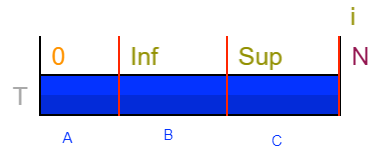
\includegraphics[width = 10cm]{invariant_EBZ952.png}
\newline
\noindent
\newline
Avec :\\\indent
A -> Déjà parcouru (sup \neq MAXPOS(T,0,inf) et \; inf \neq MINPOS(T,0,inf))\\\indent
B -> $$sum$ = SUM(T, Inf, Sup) , $inf$  = MINPOS(T,0,N)  et  $sup$  = MAXPOS(T,0,N)$\\\indent
C -> $Déjà parcouru (sup \neq MAXPOS(T,0,N) et \; inf \neq MINPOS(T,0,N)) $

\subsection{Représentation de l'invariant graphique}
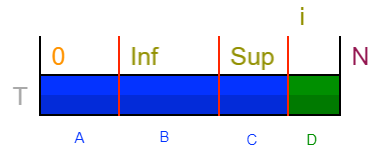
\includegraphics[width = 10 cm]{invariant.png}
\newline
\noindent

Avec :\\\indent
A ->  Déjà parcouru (sup \neq MAXPOS(T,0,inf) et \; inf \neq MINPOS(T,0,inf))\\\indent
B -> $$sum$ \; = SUM(T, Inf, Sup), inf = MINPOS(T, 0, i)  et sup = MAXPOS(T, 0, i)$\\\indent 
C -> $$new\_sum$ = NEWSUM(T,N,inf,sup)$ \\\indent 
D -> $Reste à parcourir$ 


\subsection{Invariant Formel}
\raggedright
T = T_0 \wedge  N =  N_0 \wedge 0 \leq inf \leq sup \leq N \wedge new\_sum = NEWSUM(T,N,min\_pos,max\_pos)  \wedge  $max\_pos$  = MAXPOS(T, 0, i) \wedge  $min\_pos$  = MINPOS(T, 0, i)
\wedge sum = SUM(T,N,min\_pos,max\_pos)


% !TEX root = ./main.tex
%%%%%%%%%%%%%%%%%%%%%%%%%%%%%%%%%%%%%%%%%%%%%%%%%%%%%%%%%%%%%%%%%%%%%%%%%%%%%%%%%%%%%%%%%%
% Dans cette section, il est demandé d'appliquer l'approche constructive pour la         %
% construction de votre code.                                                            %
%                                                                                        %
% Pour chaque Sous-Problème (une sous-section/SP):                                       %
% - {Pré} INIT {INV}                                                                     %
% - déterminer le Critère d'Arrêt (et donc le Gardien de Boucle)                         %
% - {INV & B} ITER {INV}                                                                 %
% - {INV & !B} END {Post}                                                                %
% - Fonction de Terminaison (pensez à justifier sur base de l'Invariant Graphique)       %
% (une sous-sous-section/tiret)                                                          %
%%%%%%%%%%%%%%%%%%%%%%%%%%%%%%%%%%%%%%%%%%%%%%%%%%%%%%%%%%%%%%%%%%%%%%%%%%%%%%%%%%%%%%%%%%
\section{Approche Constructive}
%%%%%%%%%%%%%%%%%%%%%%%%%%%%%%%%
\begin{itemize}
\item[\textbullet] Spécification du problème général
\end{itemize}
\begin{lstlisting}
/*
(>\coms{$ * $@pre$: $\;$ T $\;$ $initialisé$ $\;$ \wedge $\;$ N > 0 \wedge min\_pos $\;$ $initialisé$ $\;$ \wedge $\;$ max\_pos $\;$ $initialisé$ \newline * $@post$ : 
$\;$ $T = T_0 $\;$ \wedge $\;$ $N = N_0$ $\;$ \wedge $\;$ somme = SUM(T,N,min\_pos,max\_pos) $}<)
*/
int somme(T,N,*min_pos,*max_pos);
\end{lstlisting}
\newline
\begin{itemize}
    \item[\textbullet] Approche constructive
\newline
\end{itemize}
\begin{lstlisting}
    int somme(T,N,*min_pos,*max_pos){
    assert(T != NULL && N > 0 && min_pos != NULL && max_pos != NULL);
    //PRE $\equiv$ $T$ initialisé $\wedge$ $N > 0$ $\wedge$ $min\_pos$ init $\wedge$ $max\_pos$ init
    
    int min = T[0];
    // $T$ = $T_0$ $\wedge$ $N$ = $N_0$ $\wedge$ $min = T[0]$
    int max = T[0];
     // $T$ = $T_0$ $\wedge$ $N$ = $N_0$ $\wedge$ $min = T[0]$ $\wedge$ $max = T[0]$
    int sum = T[0];
    // $T$ = $T_0$ $\wedge$ $N$ = $N_0$ $\wedge$ $min = T[0]$ $\wedge$ $max = T[0]$ $\wedge$ $sum = T[0]$
    int new_sum = 0;
    // $T$ = $T_0$ $\wedge$ $N$ = $N_0$ $\wedge$ $min = T[0]$ $\wedge$ $max = T[0]$ $\wedge$ $sum = T[0]$ $\wedge$ $new\_sum = 0$
    *min_pos = *max_pos = 0;
    /*
    (>\coms{$T$ = $T_0$ $\wedge$ $N$ = $N_0$ $\wedge$ $min = T[0]$ $\wedge$ $max = T[0]$ $\wedge$ $sum = T[0]$}<)
    (>\coms{$\wedge$ $new\_sum = 0$ $\wedge$ $*min\_pos = 0$ $\wedge$ $*max\_pos = 0$}<)
    */
    int i = 0;
    /*
    (>\coms{$T$ = $T_0$ $\wedge$ $N$ = $N_0$ $\wedge$ $min = T[0]$ $\wedge$ $max = T[0]$ $\wedge$ $sum = T[0]$ }<)
    (>\coms{$\wedge$ $new\_sum = 0$ $\wedge$ $*min\_pos = 0$ $\wedge$ $*max\_pos = 0$ $\wedge$ $i = 0$}<)
    (>\coms{$=> *min\_pos = MINPOS(T,0,0) = MINPOS(T,inf,sup)$ $\wedge$ }<)
    (>\coms{$*max\_pos = MAXPOS(T,0,0) = MAXPOS(T,inf,sup)$}<)
    (>\coms{$\wedge$ $sum = SUM(T,1,0,0) = SUM(T,1,inf,sup)$}<)
    (>\coms{$\wedge$ $new\_sum = NEWSUM(T,1,min\_pos,max\_pos) = NEWSUM(T,1,inf,sup)$}<)
    */
    /*
    (>\coms{$INV$ $\equiv$ $N = N_0$ $\wedge$ $T = T_0$ $\wedge$ $0$ $\leq$ $inf$ $\leq$ $sup$ $\leq$ $i$ $\leq$ $N$  $\wedge$ $*min\_pos = MINPOS(T,0,i)$ }<)
    (>\coms{$\wedge$  $*max\_pos = MAXPOS(T,0,i)$ $\wedge$ $sum = SUM(T,i+1,*min\_pos,*max\_pos)$}<)
    (>\coms{$\wedge$ $new\_sum = NEWSUM(T,i+1,*min\_pos,*max\_pos)$}<)
    */
    while(i < N){
    /*
    (>\coms{$INV$ $\wedge$ $B$ $\equiv$ $N = N_0$ $\wedge$ $T = T_0$ $\wedge$ $0$ $\leq$ $inf$ $\leq$ $sup$ $\leq$ $i$ $\leq$ $N-1$ $\wedge$ $*min\_pos = MINPOS(T,0,i)$ }<)
    (>\coms{$\wedge$  $*max\_pos = MAXPOS(T,0,i)$ $\wedge$ $sum = SUM(T,i+1,*min\_pos,*max\_pos)$}<)
    (>\coms{$\wedge$ $new\_sum = NEWSUM(T,i+1,*min\_pos,*max\_pos)$}<)
    */
    new_sum += T[i];
    /*
    (>\coms{$N = N_0$ $\wedge$ $T = T_0$ $\wedge$ $0$ $\leq$ $inf$ $\leq$ $sup$ $\leq$ $i$ $\leq$ $N-1$ $\wedge$ $*min\_pos = MINPOS(T,0,i)$ }<)
    (>\coms{$\wedge$  $*max\_pos = MAXPOS(T,0,i)$ $\wedge$ $sum = SUM(T,i+1,*min\_pos,*max\_pos)$}<)
    (>\coms{$\wedge$ $new\_sum = NEWSUM(T,i+2,*min\_pos,*max\_pos)$}<)
    */
     if(T[i] < min){
     /*
     (>\coms{$N = N_0$ $\wedge$ $T = T_0$ $\wedge$ $0$ $\leq$ $inf$ $\leq$ $sup$ $\leq$ $i$ $\leq$ $N-1$ $\wedge$ $*min\_pos = MINPOS(T,0,i)$}<)
     (>\coms{$\wedge$  $*max\_pos = MAXPOS(T,0,i)$ $\wedge$ $sum = SUM(T,i+1,*min\_pos,*max\_pos)$}<)
     (>\coms{$\wedge$ $new\_sum = NEWSUM(T,i+2,*min\_pos,*max\_pos)$ $\wedge$ $T[i] < min$}<)
     */
          if(*max_pos <= *min_pos)
            /*
            (>\coms{$N = N_0$ $\wedge$ $T = T_0$ $\wedge$ $0$ $\leq$ $inf$ $\leq$ $sup$ $\leq$ $i$ $\leq$ $N-1$ $\wedge$ $*min\_pos = MINPOS(T,0,i)$}<)
            (>\coms{$\wedge$  $*max\_pos = MAXPOS(T,0,i)$ $\wedge$ $sum = SUM(T,i+1,*min\_pos,*max\_pos)$}<)
            (>\coms{$\wedge$ $new\_sum = NEWSUM(T,i+2,*min\_pos,*max\_pos)$ $\wedge$ $T[i] < min$}<) 
            (>\coms{$\wedge$ $*max\_pos$ $\leq$ $*min\_pos$}<)
            */
            sum += new_sum - T[*min_pos];
            /*
            (>\coms{$N = N_0$ $\wedge$ $T = T_0$ $\wedge$ $0$ $\leq$ $inf$ $\leq$ $sup$ $\leq$ $i$ $\leq$ $N-1$ $\wedge$ $*min\_pos = MINPOS(T,0,i)$}<)
            (>\coms{$\wedge$  $*max\_pos = MAXPOS(T,0,i)$}<)
            (>\coms{$\wedge$ $new\_sum = NEWSUM(T,i+2,*min\_pos,*max\_pos)$ $\wedge$ $T[i] < min$}<) 
            (>\coms{$\wedge$ $*max\_pos$ $\leq$ $*min\_pos$ $\wedge$ $sum = SUM(T, i+1, *min\_pos, *max\_pos)  +$}<)
            (>\coms{($new\_sum$ - $T[*min\_pos])$}<)
            */

          else
            /*
            (>\coms{$N = N_0$ $\wedge$ $T = T_0$ $\wedge$ $0$ $\leq$ $inf$ $\leq$ $sup$ $\leq$ $i$ $\leq$ $N-1$ $\wedge$ $*min\_pos = MINPOS(T,0,i)$}<)
            (>\coms{$\wedge$  $*max\_pos = MAXPOS(T,0,i)$ $\wedge$ $sum = SUM(T,i+1,*min\_pos,*max\_pos)$}<)
            (>\coms{$\wedge$ $new\_sum$ = NEWSUM(T,i+2,*min\_pos,*max\_pos) $\wedge$ $T[i] < min$ $\wedge$ $*max\_pos$ > $*min\_pos$}<) 
            */
            
            sum = new_sum;
            /*
            (>\coms{$N = N_0$ $\wedge$ $T = T_0$ $\wedge$ $0$ $\leq$ $inf$ $\leq$ $sup$ $\leq$ $i$ $\leq$ $N-1$ $\wedge$ $*min\_pos = MINPOS(T,0,i)$}<)
            (>\coms{$\wedge$  $*max\_pos = MAXPOS(T,0,i)$$\wedge$ $new\_sum = NEWSUM(T,i+2,*min\_pos,*max\_pos)$}<)
            (>\coms{$\wedge$ $T[i] < min$ $\wedge$ $*max\_pos$ > $*min\_pos$ $\wedge$ sum = $new\_sum$}<) 
            */
    
    new_sum = T[i];
    /*
     (>\coms{$N = N_0$ $\wedge$ $T = T_0$ $\wedge$ $0$ $\leq$ $inf$ $\leq$ $sup$ $\leq$ $i$ $\leq$ $N-1$ $\wedge$ $*min\_pos = MINPOS(T,0,i)$}<)
     (>\coms{$\wedge$  $*max\_pos = MAXPOS(T,0,i)$ $\wedge$ $sum = SUM(T,i+1,*min\_pos,*max\_pos)$}<)
     (>\coms{$\wedge$ $new\_sum = T[i]$ $\wedge$ $T[i] < min$}<)
     */
    min = T[i];
    /*
     (>\coms{$N = N_0$ $\wedge$ $T = T_0$ $\wedge$ $0$ $\leq$ $inf$ $\leq$ $sup$ $\leq$ $i$ $\leq$ $N-1$ $\wedge$ $*min\_pos = MINPOS(T,0,i)$}<)
     (>\coms{$\wedge$  $*max\_pos = MAXPOS(T,0,i)$ $\wedge$ $sum = SUM(T,i+1,*min\_pos,*max\_pos)$}<)
     (>\coms{$\wedge$ $new\_sum = T[i]$ $\wedge$ $T[i] < min$ $\wedge$ $min = T[i]$}<)
     */
    *min_pos = i;
    /*
     (>\coms{$N = N_0$ $\wedge$ $T = T_0$ $\wedge$ $0$ $\leq$ $inf$ $\leq$ $sup$ $\leq$ $i$ $\leq$ $N-1$}<)
     (>\coms{$\wedge$  $*max\_pos = MAXPOS(T,0,i)$ $\wedge$ $sum = SUM(T,i+1,i,*max\_pos)$}<)
     (>\coms{$\wedge$ $new\_sum = T[i]$ $\wedge$ $T[i] < min$ $\wedge$ $min = T[i]$ $\wedge$ $*min\_pos = i$}<)
     */
    }
     if(T[i] > max){
     /*
     (>\coms{$N = N_0$ $\wedge$ $T = T_0$ $\wedge$ $0$ $\leq$ $inf$ $\leq$ $sup$ $\leq$ $i$ $\leq$ $N-1$ $\wedge$ $*min\_pos = MINPOS(T,0,i)$}<)
     (>\coms{$\wedge$  $*max\_pos = MAXPOS(T,0,i)$ $\wedge$ $sum = SUM(T,i+1,*min\_pos,*max\_pos)$}<)
     (>\coms{$\wedge$ $new\_sum = NEWSUM(T,i+2,*min\_pos,*max\_pos)$ $\wedge$ $T[i] > max$}<)
     */
          if(*min_pos <= *max_pos)
            /*
            (>\coms{$N = N_0$ $\wedge$ $T = T_0$ $\wedge$ $0$ $\leq$ $inf$ $\leq$ $sup$ $\leq$ $i$ $\leq$ $N-1$ $\wedge$ $*min\_pos = MINPOS(T,0,i)$}<)
            (>\coms{$\wedge$  $*max\_pos = MAXPOS(T,0,i)$ $\wedge$ $sum = SUM(T,i+1,*min\_pos,*max\_pos)$}<)
            (>\coms{$\wedge$ $new\_sum = NEWSUM(T,i+2,*min\_pos,*max\_pos)$ $\wedge$ $T[i] > max$}<)
            (>\coms{$\wedge$ $*min\_pos$ $\leq$ $*max\_pos$}<)
            */
            sum += new_sum - T[*max_pos];
            /*
            (>\coms{$N = N_0$ $\wedge$ $T = T_0$ $\wedge$ $0$ $\leq$ $inf$ $\leq$ $sup$ $\leq$ $i$ $\leq$ $N-1$ $\wedge$ $*min\_pos = MINPOS(T,0,i)$}<)
            (>\coms{$\wedge$  $*max\_pos = MAXPOS(T,0,i)$}<)
            (>\coms{$\wedge$ $new\_sum = NEWSUM(T,i+2,*min\_pos,*max\_pos)$ $\wedge$ $T[i] > max$}<)
            (>\coms{$\wedge$ $*min\_pos$ $\leq$ $*max\_pos$ $\wedge$ $sum = SUM(T,i+1, $*min\_pos$, $*max\_pos$)$ +}<)
            (>\coms{($new\_sum$ - $T[*max\_pos])$}<)
            */

          else
          /*
            (>\coms{$N = N_0$ $\wedge$ $T = T_0$ $\wedge$ $0$ $\leq$ $inf$ $\leq$ $sup$ $\leq$ $i$ $\leq$ $N-1$ $\wedge$ $*min\_pos = MINPOS(T,0,i)$}<)
            (>\coms{$\wedge$  $*max\_pos = MAXPOS(T,0,i)$ $\wedge$ $sum = SUM(T,i+1,*min\_pos,*max\_pos)$}<)
            (>\coms{$\wedge$ $new\_sum$ = $NEWSUM(T,i+2,*min\_pos,*max\_pos)$ $\wedge$ $T[i] > max$ $\wedge$ $*min\_pos$ > $*max\_pos$}<) 
            */
            sum  = new_sum
            /*
            (>\coms{$N = N_0$ $\wedge$ $T = T_0$ $\wedge$ $0$ $\leq$ $inf$ $\leq$ $sup$ $\leq$ $i$ $\leq$ $N-1$ $\wedge$ $*min\_pos = MINPOS(T,0,i)$}<)
            (>\coms{$\wedge$  $*max\_pos = MAXPOS(T,0,i)$ $\wedge$ $new\_sum$ = $NEWSUM(T,i+2,*min\_pos,*max\_pos)$}<)
            (>\coms{ $\wedge$ $T[i] > max$ $\wedge$ $*min\_pos$ > $*max\_pos$ $\wedge$ sum = $new\_sum$}<) 
            */

    new_sum = T[i];
    /*
     (>\coms{$N = N_0$ $\wedge$ $T = T_0$ $\wedge$ $0$ $\leq$ $inf$ $\leq$ $sup$ $\leq$ $i$ $\leq$ $N-1$ $\wedge$ $*min\_pos = MINPOS(T,0,i)$}<)
     (>\coms{$\wedge$  $*max\_pos = MAXPOS(T,0,i)$ $\wedge$ $sum = SUM(T,i+1,*min\_pos,*max\_pos)$}<)
     (>\coms{$\wedge$ $new\_sum = T[i]$ $\wedge$ $T[i] > max$}<)
     */
    max = T[i];
    /*
     (>\coms{$N = N_0$ $\wedge$ $T = T_0$ $\wedge$ $0$ $\leq$ $inf$ $\leq$ $sup$ $\leq$ $i$ $\leq$ $N-1$ $\wedge$ $*min\_pos = MINPOS(T,0,i)$}<)
     (>\coms{$\wedge$  $*max\_pos = MAXPOS(T,0,i)$ $\wedge$ $sum = SUM(T,i+1,*min\_pos,*max\_pos)$}<)
     (>\coms{$\wedge$ $new\_sum = T[i]$ $\wedge$ $T[i] > max$ $\wedge$ $max = T[i]$}<)
    */
    *max_pos = i;
    /*
     (>\coms{$N = N_0$ $\wedge$ $T = T_0$ $\wedge$ $0$ $\leq$ $inf$ $\leq$ $sup$ $\leq$ $i$ $\leq$ $N-1$ $\wedge$ $*min\_pos = MINPOS(T,0,i)$}<)
     (>\coms{$\wedge$ $sum = SUM(T,i+1,*min\_pos,i)$}<)
     (>\coms{$\wedge$ $new\_sum = T[i]$ $\wedge$ $T[i] > max$ $\wedge$ $max = T[i]$ $\wedge$ $*max\_pos$ = i}<)
    */
    }
    i++;
    /*
    (>\coms{$INV$ $\equiv$ $0$ $\leq$ $i$ $\leq$ $N$ $\wedge$ $T = T_0$ $\wedge$ $N = N_0$}<)
    (>\coms{$\wedge$ $*min\_pos = MINPOS(T,0,i+1)$ }<)
    (>\coms{$\wedge$  $*max\_pos = MAXPOS(T,0,i+1)$ $\wedge$ $sum = SUM(T,i+2,*min\_pos,*max\_pos)$}<)
    (>\coms{ $\wedge$ $new\_sum = NEWSUM(T,i+3,*min\_pos,*max\_pos)$}<)
    */
    }
    /*
    (>\coms{$INV$ $\wedge$ $\neg$ $B$ $\equiv$ $i == N$ $\wedge$ $T = T_0$ $\wedge$ $N = N_0$ }<)
    (>\coms{$\wedge$ $*min\_pos = MINPOS(T,0,N)$ }<)
    (>\coms{$\wedge$  $*max\_pos = MAXPOS(T,0,N)$ $\wedge$ $sum = SUM(T,N,*min\_pos,*max\_pos)$}<)
    (>\coms{$\wedge$ $new\_sum = NEWSUM(T,N,*min\_pos,*max\_pos)$}<)
    */
    return sum; (>\label{code:ret}<)
    /*
    (>\coms{$POST$ $\equiv$ $T = T_0$ $\wedge$ $N = N_0$ $\wedge$ $sum = SUM(T,inf,sup)$ }<)
    (>\coms{$\wedge$ $*max\_pos = MAXPOS(T,0,N)$ $\wedge$ $*min\pos = MINPOS(T,0,N)$}<)
}   */
\end{lstlisting}


% !TEX root = ./main.tex
%%%%%%%%%%%%%%%%%%%%%%%%%%%%%%%%%%%%%%%%%%%%%%%%%%%%%%%%%%%%%%%%%%%%%%%%%%%%%%%%%%%%%%%%%%
% Dans cette section, indiquez le code complet (sans assertions intermédiaires) de votre %
% solution                                                                               %
%%%%%%%%%%%%%%%%%%%%%%%%%%%%%%%%%%%%%%%%%%%%%%%%%%%%%%%%%%%%%%%%%%%%%%%%%%%%%%%%%%%%%%%%%%
\section{Code Complet}\label{code}
%%%%%%%%%%%%%%%%%%%%%%%
\begin{lstlisting}[caption={somme.c}]
int somme(T,N,*min_pos,*max_pos){
    assert(T != NULL && N > 0 && min_pos != NULL && max_pos != NULL)
    int min = T[0];
    int max = T[0];
    int sum = T[0];
    int new_sum = 0;
    *min_pos = *max_pos = 0;

    int i = 0;
    while(i < N){
     new_sum += T[i];

     if(T[i] < min){
        if(*max_pos <= *min_pos)
            sum += new_sum - T[*min_pos];

        else
            sum = new_sum;

         new_sum = T[i];
         min = T[i];
         *min_pos = i;
     }
     if(T[i] > max){
        if(*min_pos <= *max_pos)
            sum += new_sum - T[*max_pos];

        else
            sum  = new_sum

        new_sum = T[i];
        max = T[i];
       *max_pos = i;
     }
    i++;
    }
    
    return sum; (>\label{code:ret}<)
}
\end{lstlisting}

% !TEX root = ./main.tex
%%%%%%%%%%%%%%%%%%%%%%%%%%%%%%%%%%%%%%%%%%%%%%%%%%%%%%%%%%%%%%%%%%%%%%%%%%%%%%%%%%%%%%%%%%
% Dans cette section, vous devez étudier complètement la complexité de votre code.       %
% Soyez le plus formel (i.e., mathématique) possible.                                    %
%%%%%%%%%%%%%%%%%%%%%%%%%%%%%%%%%%%%%%%%%%%%%%%%%%%%%%%%%%%%%%%%%%%%%%%%%%%%%%%%%%%%%%%%%%
\section{Complexité}\label{complexite}
%%%%%%%%%%%%%%%%%%%%
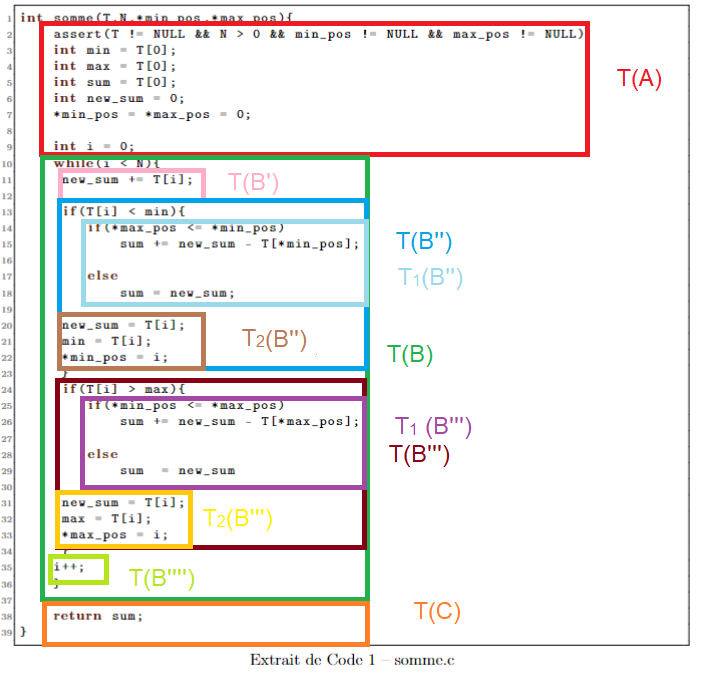
\includegraphics[width = 15 cm]{complexite.png}
\begin{enumerate}
    \item[-] Par application des règles 2 et 6 : 
    \[T(N) = T(A) + T(B) + T(C)\]
    \item[-] Par application des règles 1 et 5 : 
    \[T(N) = 8 + \sum_{i = 0}^{N-1} {(T(B') + T(B'') + T(B''') + T(B''''))} + 1\]
    \[T(N) = 8 + \sum_{i = 0}^{N-1} {(1 + T(B'') + T(B''') + 1)} + 1\]
    \item[-] Quid de T(B'') ? 
    \[T(B'') = T_1(B'') + T_2(B'')\]
    \item[-] Quid de $T_1$ (B'') ? Par application de la règle 3 :
    \[T_1(B'') = max(T_{if}(), T_{else}())\]
    \[T_{if}() = 1\] et \[T_{else}() = 1\] donc
    \[T_1(B'') = 1\]
    \item[-] Quid de $T_2$(B'') ? Par application de la règle 2 :
    \[T_2(B'') = 3\]
    \item[-] Ainsi T(B'') devient : 
    \[T(B'') = 1 + 3\]
    \[T(B'') = 4\]
    \item[-] Quid de T(B''') ?
    \[T(B''') = T_1(B''') + T_2(B''')\]
    \item[-] Quid de $T_1$(B''') ? Par application de la règle 3:
    \[T_1(B''') = max(T_{if}(), T_{else}())\]
    \[T_{if}() = 1\] et \[T_{else}() = 1\] donc
    \[T_1(B''') = 1\]
    \item[-] Quid de $T_2$(B''') ? Par application de la règle 2 :
    \[T_2(B''') = 3\]
    \item[-] Ainsi T(B''') devient : 
    \[T(B''') = 1 + 3\]
    \[T(B''') = 4\]
    \item[-] Ainsi T(B) devient : 
    \[\[T(B) = \sum_{i = 0}^{N-1} {10} = 10N\]\]
    \item[-] Donc:
    \[T(N) = 8 + 10N + 1 = 9 + 10N\]
    \item[-] Par quoi borner T(N) ?
    \[O(n)\] complexité linéaire.
\end{enumerate}
Preuve ?\\\indent
But : Trouver une constante \textit{c} $\in \math{R^+}$ et un seuil $n_0$ à partir duquel $T(n_0)$ $\leq$ $c$ x $n_0$.
\\\indent On remarque que pour $c = 11$ et $n_0$ = 9 on a $\forall n \geq n_0$: c x n $\geq$ 9 + 10N\\
\underline{exemple:}\begin{enumerate}
    \item[-] si n = 9 : 99 $\geq$ 99
    \item[-] si n = 10 : 110 $\geq$ 109
    \item[-] si n = 11 : ...
\end{enumerate}

% !TEX root = ./main.tex
%%%%%%%%%%%%%%%%%%%%%%%%%%%%%%%%%%%%%%%%%%%%%%%%%%%%%%%%%%%%%%%%%%%%%%%%%%%%%%%%%%%%%%%%%%
% Rédigez ici la conclusion de votre rapport.                                            %
%%%%%%%%%%%%%%%%%%%%%%%%%%%%%%%%%%%%%%%%%%%%%%%%%%%%%%%%%%%%%%%%%%%%%%%%%%%%%%%%%%%%%%%%%%
\section{Conclusion}\label{conclusion}
%%%%%%%%%%%%%%%%%%%%%
Il est donc possible de résoudre ce problème en O(N) (i.e en une seule boucle) 

%%%%%%%%%%%%%%%%%%%% FIN DE LA ZONE PROTÉGÉE %%%%%%%%%%%%%%%%%%%%

\end{document}
